%!TEX program = xelatex

\documentclass{article}

% if you need to pass options to natbib, use, e.g.:
%     \PassOptionsToPackage{numbers, compress}{natbib}
% before loading neurips_2021

% ready for submission
\usepackage[final]{neurips_2021}

% to compile a preprint version, e.g., for submission to arXiv, add add the
% [preprint] option:
%     \usepackage[preprint]{neurips_2021}

% to compile a camera-ready version, add the [final] option, e.g.:
%     \usepackage[final]{neurips_2021}

% to avoid loading the natbib package, add option nonatbib:
%    \usepackage[nonatbib]{neurips_2021}

\usepackage[utf8]{inputenc} % allow utf-8 input
\usepackage[T1]{fontenc}    % use 8-bit T1 fonts
\usepackage{hyperref}       % hyperlinks
\usepackage{url}            % simple URL typesetting
\usepackage{booktabs}       % professional-quality tables
\usepackage{amsfonts}       % blackboard math symbols
\usepackage{nicefrac}       % compact symbols for 1/2, etc.
\usepackage{microtype}      % microtypography
\usepackage{xcolor}         % colors
\usepackage[UTF8]{ctex}
\usepackage{graphicx}
\usepackage{amsthm}
\usepackage{multirow}
\newtheorem{definition}{定义}
\newtheorem{theorem}{定理}
\usepackage{subcaption}
\usepackage[export]{adjustbox}

\setCJKmainfont{SimSun}[AutoFakeBold=2.5,ItalicFont=KaiTi]%
\setCJKsansfont{SimHei}[AutoFakeBold=2.5]%
\setCJKmonofont{FangSong}%


\title{《最优化方法》上机作业1:线搜索、牛顿法与拟牛顿法数值实验}

% The \author macro works with any number of authors. There are two commands
% used to separate the names and addresses of multiple authors: \And and \AND.
%
% Using \And between authors leaves it to LaTeX to determine where to break the
% lines. Using \AND forces a line break at that point. So, if LaTeX puts 3 of 4
% authors names on the first line, and the last on the second line, try using
% \AND instead of \And before the third author name.

\author{%
  张旻昊 Minhao Zhang 2101213233 \\
  前沿交叉学科研究院 Academy for Advanced Interdisciplinary Studies\\
  北京大学 Peking University\\
  颐和园路5号,海淀,北京 Yiheyuan Rd. $5^{th}$, Haidian, Beijing\\
  \texttt{minhaozhang@pku.edu.cn} \\
  % examples of more authors
  % \And
  % Coauthor \\
  % Affiliation \\
  % Address \\
  % \texttt{email} \\
  % \AND
  % Coauthor \\
  % Affiliation \\
  % Address \\
  % \texttt{email} \\
  % \And
  % Coauthor \\
  % Affiliation \\
  % Address \\
  % \texttt{email} \\
  % \And
  % Coauthor \\
  % Affiliation \\
  % Address \\
  % \texttt{email} \\
}

\begin{document}
%\begin{CJK*}{UTF8}{gbsn}

\maketitle

\begin{abstract}
  本实验实现了线搜索、Newton方法及拟Newton方法的程序(各包括多种算法),并利用Ackley函数测试各种牛顿型方法的收敛性能、精度等数值表现,此外还进一步分析了线搜索及初始值对收敛过程的影响。
  
\end{abstract}

\section{实验设定}
\subsection{目标函数选取}
\begin{figure}[h]
  \centering
  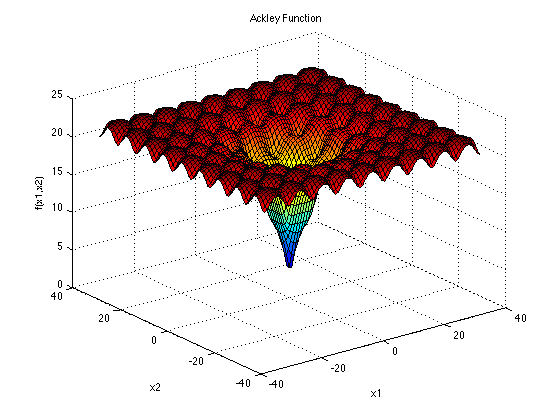
\includegraphics[width=.65\linewidth]{pics/ackley.png}
  \caption{二维Ackley函数的可视化}
  \label{fig:ackley}
\end{figure}

本实验通过Ackley函数评估不同方法,其形式如下:
\[ \texttt{Ackley}(x) = -20 exp[-\frac{1}{5} \sqrt{\frac{1}{n}\sum\limits_{i=1}^n x_i^2}] - exp[\frac{1}{n} \sum\limits_{i=1}^n cos(2\pi x_i)] + 20+e \]

Ackley函数具有全局最小值$x^* = (0,0,...,0), f(x^*)=0$,此外它还有众多极小值,其二维形式如图\ref{fig:ackley}所示,我们的算法旨在找到其中任一个局部极小值点。

\subsection{线搜索算法}
本实验实现了两类线搜索算法:
\begin{itemize}
  \item \textbf{精确线搜索}。采用Fibonacci法进行精确线搜索,算法过程如图\ref{fig:fib_algo}所示。在实验中,首先利用进退法获取初始搜索区间;此后进行Fibonacci搜索,给定函数调用次数n,利用此方法迭代n-1次即可获取精确搜索区间,我们取此区间的中点作为搜索结果$\alpha$。默认情况下,本文的实验设置$n=20$,进退法的初始步长$\alpha_0=2$,步长变化量$step=1$,步长扩大因子$mag=2$。
  \begin{figure}[h]
    \centering
    \includegraphics[width=.8\linewidth]{pics/fib_algo.jpg}
    \caption{Fibonacci搜索算法}
    \label{fig:fib_algo}
  \end{figure}
  \item \textbf{非精确线搜索}。
\end{itemize}



\subsection{Newton方法}

\subsection{拟Newton方法}

本报告处理词汇相关度问题,给定两个单词$w_1$和$w_2$,需要对其在语义上的相关程度给出0-5的打分,分数越高代表越相关。如表\ref{tab:dataset_eg}所示,在语义上有更强关联(同义词,指代同种或类似概念)的词对具有更高的打分。

\begin{table*}[h]
  \centering
  \begin{tabular}{c c c}
    \toprule
    \bfseries Word 1 & \bfseries Word2 & \bfseries Similarity \\
    \cmidrule(lr){1-3}
    female & woman & 4.96 \\
    finger & toe & 3.76 \\
    flyer & justice & 1.18\\
    \bottomrule
  \end{tabular}
  \caption{词汇相关度数据示例,数据源于MTURK-771数据集}
  \label{tab:dataset_eg}
\end{table*}

\section{方法概览}
本文使用基于字典和语料的两类方法计算关联度。
\subsection{基于字典计算相关度}
此类方法基于Wordnet,对于上述两个单词,分别在Wordnet种找到其同义集合,并根据这一对集合中的所有结点在Wordnet中的相对路径计算相似度(例如,集合间的最短路径越短,Path相似度越高)。

在实现中,本文使用\texttt{nltk}构建Wordnet,通过其\texttt{synset}方法获取同义集,这样即可在集合上获取结点并利用\texttt{path\_similarity}、\texttt{res\_similarity}、\texttt{lin\_similarity}和\texttt{jcn\_similarity}方法计算相似度指标。特别地,注意到Path和Lin相似度都是0-1之间,直接将其乘5作为输出;由于Resnik和J-C可能产生正无穷值,实验中将所有无穷值替换为最大的有意义值,再线性放缩到0-5的区间中(例如最大值是12,则将所有值乘以5/12)作为输出。另外,由于后三种相似度需要在语料上统计频率,这里使用nltk默认的\texttt{brown}语料库。

\subsection{基于语料计算相关度}
本文使用word2vec算法在语料上训练词向量,在根据词向量的cosine相似度作为相关程度预测。具体地,本文使用gensim库训练词向量,语料使用text8。得到$w_1$和$w_2$的词向量$\mathbf{v_1}, \mathbf{v_2}$后,利用下式计算相似度。
\[ sim(w_1, w_2) := \frac{\mathbf{v_1}\cdot \mathbf{v_2}}{|\mathbf{v_1}|\cdot |\mathbf{v_2}|} \]
特别地,如果词表中不存在某单词,记其词向量为零向量。

\subsection{评估方法}
本文在MTURK-771上进行评估,将上述输出的相似度$sim_{pred}^i$与数据集所给的相似度$sim_{gold}^i$比较,通过如下方法计算均方误差MSE和Spearman相关系数。
\[ MSE = \frac{1}{N} \sum\limits_{i=1}^{N} {(sim_{pred}^i-sim_{gold}^i)}^2 \]
\[ Spearman = \frac{\sum\limits_{i=1}^N (sim_{pred}^i - \overline{sim_{pred}})(sim_{gold}^i - \overline{sim_{gold}})}{\sqrt{\sum\limits_{i=1}^N {(sim_{pred}^i - \overline{sim_{pred}})}^2  \sum\limits_{i=1}^N {(sim_{gold}^i - \overline{sim_{gold}})}^2}} \]


\begin{table*}[h]
  \centering
  \begin{tabular}{c l c c}
    \toprule
    \bfseries Type & \bfseries Methods & \bfseries MSE & \bfseries Spearman\\
    \cmidrule(lr){1-4}
    \multirow{4}{*}{\bfseries I} &
    Path  & 1.884 & .497 \\
    & Resnik & 1.088 & .417 \\
    & Lin & 1.846 & .493 \\
    & J-C & 7.321 & .483 \\
    \cmidrule(lr){1-4}
    \multirow{1}{*}{\bfseries II} &
    Word2vec & \bfseries 0.867 & \bfseries .506 \\
    \bottomrule
\end{tabular}
  \caption{各类方法的表现。其中I和II分别代表基于字典和基于语料库的两类方法。}
  \label{tab:overall_eval}
\end{table*}

\section{结果分析}
\subsection{总体结果比较}
上述方法所得实验结果如表\ref{tab:overall_eval}所示,可见基于语料的Word2vec具有最优的表现,超过了所有基于字典的方法。在字典类方法中,Path和Lin相似度相对最优且较为接近,在MSE和Spearman两个指标中分别占优。

\subsection{结果分析}
\begin{itemize}
  \item 基于语料的word2vec方法效果好于所有本文中的字典类方法,这体现了通过模型学习语义的潜力,进一步扩充此方法可能达到更好的效果。
  \item 观察表\ref{tab:overall_eval}可以发现,J-C方法在MSE上表现不佳,但是Spearman相关性并不差,为解释这一点,图\ref{fig:distrib}展示了Lin、Word2vec方法所得的相似性分数分布及正确相似性打分分布。可见,Lin所得的得分普遍偏高,但可能不同词对的打分相对高低仍保持正确,这使得其MSE较高,但由于趋势与正确答案相近,Spearman相关性仍较高。同时,Word2vec得分分布较好的拟合了正确答案,因此在两个指标中都较好。这提示我们,MSE与Spearman虽都是可行的评估指标,但二者重视的方面不同(MSE重视打分分布,Spearman重视相对大小关系及趋势),使用多种指标评估我们的方法有助于更好的理解模型表现。
\end{itemize}


\begin{figure}[h]
  % \centering
  \begin{subfigure}{.42\textwidth}
    \includegraphics[width=1.\linewidth,right]{pics/gold.pdf}
    \caption{}
    \label{fig:gold}
  \end{subfigure}
  \hfill
  \begin{subfigure}{.42\textwidth}
    \includegraphics[width=1.\linewidth,left]{pics/lin.pdf}
    \caption{}
    \label{fig:lin}
  \end{subfigure}
  % \hfill
  \begin{subfigure}{.42\textwidth}
    \centering
    \includegraphics[width=1.\linewidth]{pics/w2v.pdf}
    \caption{}
    \label{fig:w2v}
  \end{subfigure}%
  \caption{相似性得分分布}
  \label{fig:distrib}
  \end{figure}


%end{CJK*}
\end{document}
